\documentclass[10pt,letterpaper]{article}
\usepackage[margin=0.7in]{geometry}
\usepackage[T1]{fontenc}
\usepackage{helvet}
\renewcommand{\familydefault}{\sfdefault}
\usepackage{graphicx,booktabs,amsmath,xcolor,fancyhdr}
\usepackage[colorlinks=true,urlcolor=teal,citecolor=teal,linkcolor=teal]{hyperref}
\definecolor{ink}{HTML}{163640}
\definecolor{teal}{HTML}{117C77}
\setlength{\parindent}{0pt}
\setlength{\parskip}{5pt}
\setlength{\headheight}{14pt}
\setlength{\tabcolsep}{5pt}
\renewcommand{\arraystretch}{1.18}
\pagestyle{fancy}\fancyhf{}
\fancyhead[L]{\small\color{ink}STORMWATER DETENTION MODELING}
\fancyhead[R]{\small Conceptual study}
\fancyfoot[L]{\footnotesize Synthetic inputs; no field calibration}
\fancyfoot[R]{\thepage\ / 6}
\newcommand{\pagetitle}[1]{\vspace*{2pt}{\Large\bfseries\color{ink}#1}\par\vspace{5pt}}
\begin{document}
\pagetitle{Parking-lot detention: a tested design comparison}
{\small Prepared for Manasi's project portfolio. Assistant-generated study; individual review remains pending.}

\textbf{Question.} What is the smallest tested storage that lowers peak downstream discharge by at least 50\%, avoids overflow, and remains below 1\% of capacity within 24 hours after rainfall ends? These are educational objectives, not local drainage requirements.

\textbf{Finding.} The smallest tested feasible capacity is 150 m$^3$: 0.75 m modeled storage depth over 200 m$^2$, with a 100 by 100 mm floor opening. Across all 50 mm storm shapes, peak reduction is at least 63.09\%, overflow is zero, and the longest drainage time is 7.81 h after rainfall ends.

\begin{center}\small
\begin{tabular}{p{0.30\linewidth}p{0.62\linewidth}}\toprule
Input & Assumption \\ \midrule
Contributing areas & Parking 4000 m$^2$ + footprint 200 m$^2$ \\
CN; abstraction; lag & 98; $I_a=0.2S$; 10 min \\
Synthetic rainfall & 25, 50, 100 mm; 60 min; 3 shapes \\
Storage and openings & 6 depths $\times$ 4 square openings \\
Initial storage; basin losses & Empty; zero infiltration and evaporation \\
Outlet coefficient; gravity & $C_d=0.62$; $g=9.80665$ m/s$^2$ \\
Final numerical resolution & 1.875 s; at least 30 h, extended if needed \\
\bottomrule\end{tabular}
\end{center}

\textbf{A consistent comparison.} The same 4200 m$^2$ contributes in every case. The baseline treats the reserved footprint as an impervious collection pad with negligible storage. Its rainfall discharges directly. Detention cases store that rainfall together with parking runoff. Both streams reach the same downstream accounting point.

\begin{center}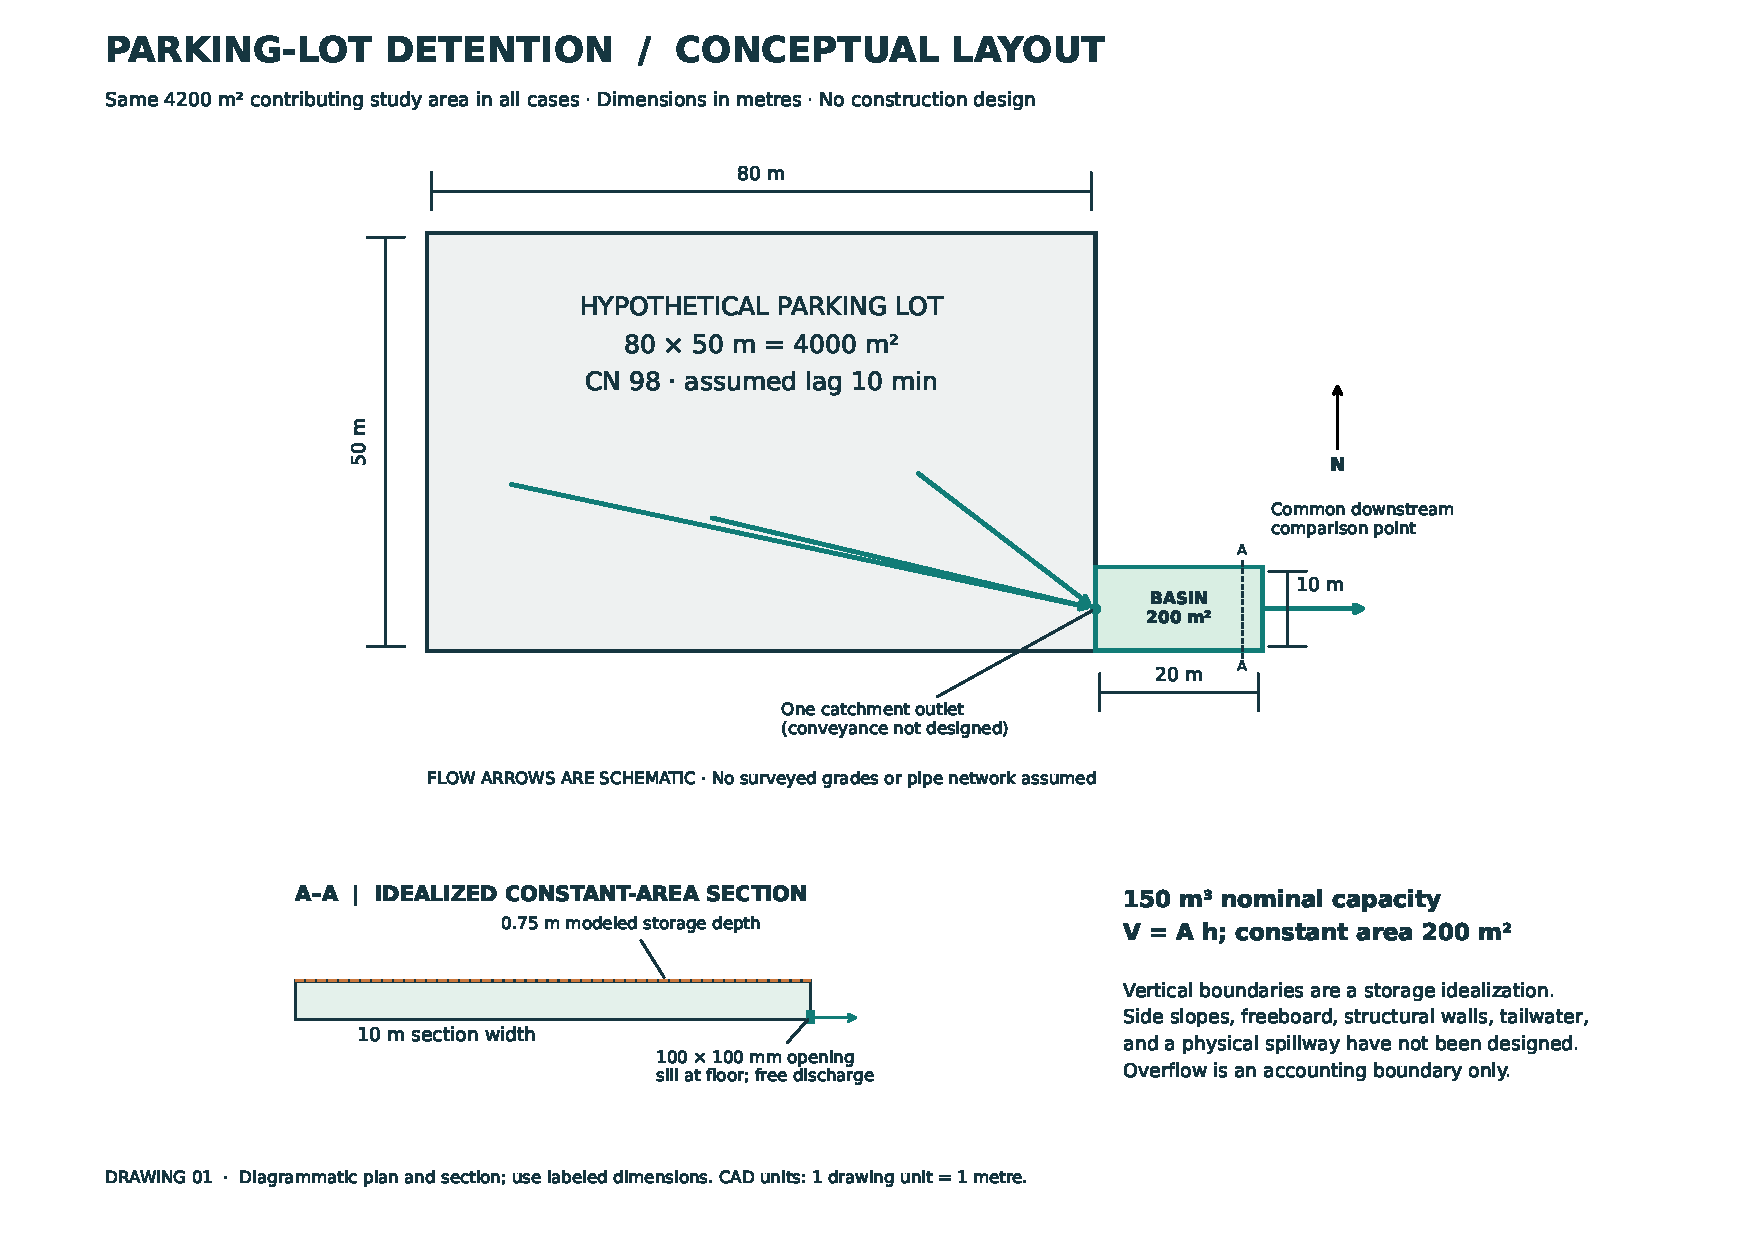
\includegraphics[width=.94\linewidth,height=3.65in,keepaspectratio]{site_plan.pdf}\end{center}
{\footnotesize Figure 1. Dimensioned conceptual geometry. The constant-area basin is a storage idealization; walls, grading, freeboard and a physical spillway are not designed. Editable SVG and metre-coordinate DXF are included.}
\newpage
\pagetitle{Method and reproducible assumptions}
\textbf{Rainfall and event losses.} Project-defined block shapes share one duration and total depth. Each shape divides the event into equal-duration blocks with relative weights: Uniform $(1,1,1,1,1,1)$; Front Loaded $(6,5,4,3,2,1)$; Back Loaded $(1,2,3,4,5,6)$. Each vector is normalized by its sum. Block boundaries are integrated exactly even if a computational interval crosses a boundary.

For cumulative precipitation $P$ and retention $S$ in millimetres, the event CN calculation is\cite{cn}
\[
S=25400/CN-254,\qquad I_a=0.2S,\qquad
P_e(P)=\begin{cases}0&P\leq I_a,\\(P-I_a)^2/(P-I_a+S)&P>I_a.\end{cases}
\]
Incremental runoff is the difference between successive cumulative $P_e$ values. It is multiplied by parking area and divided by 1,000 to obtain m$^3$. CN 100 is handled explicitly as $P_e=P$, including $P=0$. Loss state resets between independent events. No second impervious-area adjustment is made.

\textbf{Hydrograph transformation.} The 33 local reference ordinates are from TxDOT Table 4-29.\cite{ordinates} Set $T_p=t_{lag}+\Delta t/2$, relative to the beginning of an excess-rainfall pulse.\cite{uh} Integrate the piecewise-linear dimensionless curve over every output interval to form nonnegative volume fractions $w_j$ with $\sum_j w_j=1$. Convolve those fractions with runoff volumes; divide by $\Delta t$ to obtain interval-average flow. Retain the complete reference tail through $5T_p$. The lag is assumed, not estimated from a surveyed flow path. A hydrograph supplies both timing and volume needed for detention.\cite{selection}

\textbf{Storage and outlet.} Use $V=A_bh$ with fixed area. The project's free-discharge square opening has side $a$ and sill at the floor. Integrating local velocity over the wetted opening gives
\[
Q(h)=\int_0^{\min(h,a)} C_da\sqrt{2g(h-z)}\,dz
=\tfrac23 C_da\sqrt{2g}\,[h^{3/2}-\max(h-a,0)^{3/2}].
\]
This expression includes partial wetting near an empty basin. It is an idealization with constant $C_d$, not a calibrated HEC-HMS rating. The fully wetted approximation uses centroid head, $C_da^2\sqrt{2g(h-a/2)}$; it is not used below submergence.\cite{outlet}

\textbf{Implicit continuity.} For an interval input volume $I_n$, solve
\[
V_{n+1}+\Delta t\,Q(V_{n+1}/A_b)=V_n+I_n
\]
with a bracketed Brent root solver on $[0,\min(V_{max},V_n+I_n)]$. If the available volume exceeds $V_{max}+\Delta t\,Q(V_{max}/A_b)$, fix storage at capacity and count the excess as overflow. Controlled discharge plus overflow is downstream flow. This is backward Euler; it uses the level-pool conservation concept but is not the manual's trapezoidal Modified Puls algorithm.\cite{routing}

\textbf{Reporting conventions.} Flow peaks are maxima of interval-average flow; peak times are interval centers. Depth and storage use step-boundary states. Overflow onset is the beginning of its first interval. Drawdown is the final interpolated crossing below the capacity fraction, minus rainfall end time, with no later rebound. Any remaining horizon storage is retained in the water balance. Small outlets triggered horizon extension up to 60 hours. Exact emptying is asymptotic for this rating; ``drained'' means below the stated threshold.
\newpage
\pagetitle{Candidate comparison and selected-event results}
The search evaluates 24 storage--opening configurations over 9 synthetic storms (216 routed cases plus matching baselines). Every design-event shape must meet all three objectives. Rank passing designs by capacity, then shortest worst-case drawdown, then overflow, then opening size. The smallest tested feasible capacity is 150 m$^3$: 0.75 m modeled storage depth over 200 m$^2$, with a 100 by 100 mm floor opening. Across all 50 mm storm shapes, peak reduction is at least 63.09\%, overflow is zero, and the longest drainage time is 7.81 h after rainfall ends.

\begin{center}\small
\begin{tabular}{lrrrrr}\toprule
Shape & Baseline & Downstream & Reduction & Max. storage & Drawdown \\
 & L/s & L/s & \% & m$^3$ & h after rain \\\midrule
Uniform & 57.48 & 21.22 & 63.09 & 129.48 & 7.65 \\
Front Loaded & 73.19 & 21.04 & 71.25 & 127.55 & 7.51 \\
Back Loaded & 85.67 & 21.94 & 74.39 & 137.76 & 7.81 \\
\bottomrule\end{tabular}\end{center}

\begin{center}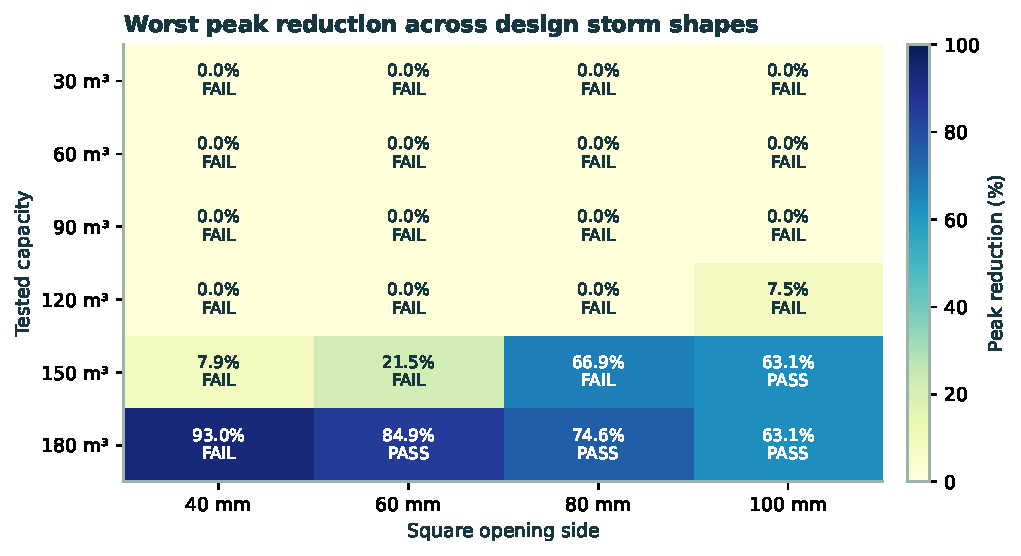
\includegraphics[width=.86\linewidth,height=2.9in,keepaspectratio]{results/figures/design_comparison.pdf}\end{center}
{\footnotesize Figure 2. Cell colour shows the worst peak reduction for the design storms. PASS requires peak, overflow and drainage criteria together. A high percentage alone is insufficient.}

\textbf{Why smaller alternatives fail.} Every lower-capacity tested design fails at least one design storm. At 120 m$^3$, even the 100 mm opening has 18.46 m$^3$ worst-case overflow. At the selected capacity, 1 of 4 tested openings pass all three shapes.

\textbf{Outside the design event.} These are stress scenarios with no assigned return periods. The selected geometry is not resized between events.
\begin{center}\small\begin{tabular}{rrrr}\toprule
Rainfall (mm) & Peak reduction range (\%) & Overflow range (m$^3$) & Longest drawdown (h) \\\midrule
25 & 54.02--67.12 & 0.00--0.00 & 6.53 \\
50 & 63.09--74.39 & 0.00--0.00 & 7.81 \\
100 & 0.00--3.21 & 162.53--173.33 & 8.02 \\
\bottomrule\end{tabular}\end{center}

The 100 mm results demonstrate finite storage limits. When the basin fills, accounting overflow can dominate downstream discharge. Overflow is not a modeled spillway flow or an inundation prediction.
\newpage
\pagetitle{Hydrographs, water depth, and the drainage tail}
\begin{center}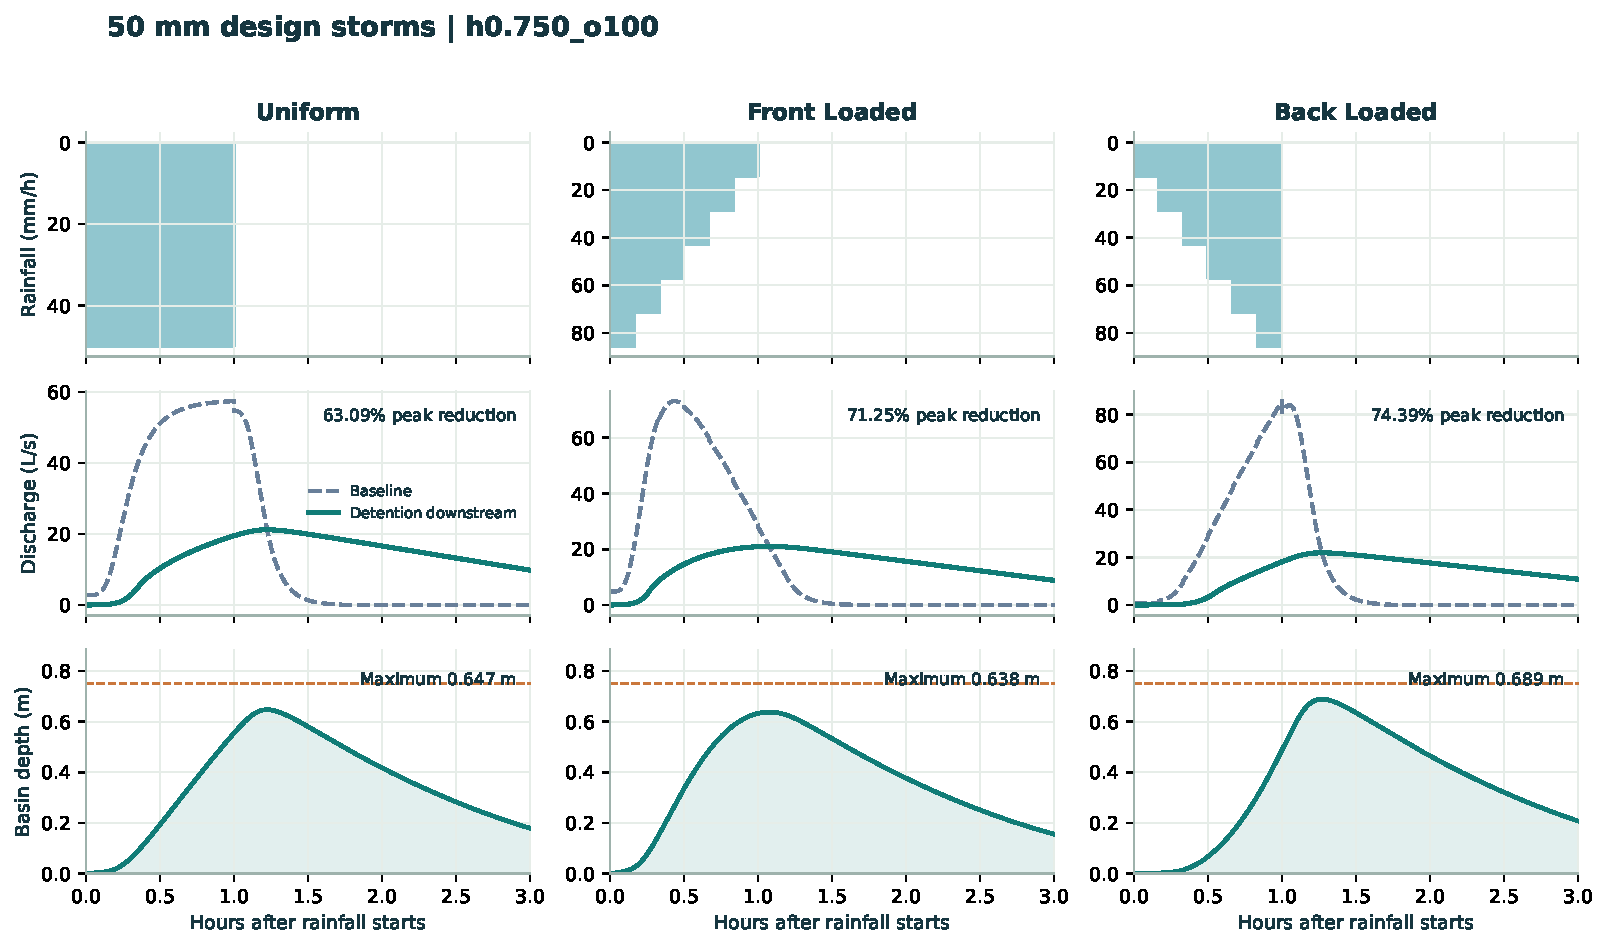
\includegraphics[width=\linewidth,height=4.0in,keepaspectratio]{results/figures/design_hydrographs.pdf}\end{center}
{\footnotesize Figure 3. Full-resolution design-event curves for h0.750\_o100. Rainfall generates a delayed inflow hydrograph; storage and controlled discharge rise together. Dashed depth marks capacity.}

The 50 mm event supplies 177.103 m$^3$ of parking runoff plus 10.000 m$^3$ of direct footprint rainfall, or 187.103 m$^3$ in total. Detention does not eliminate this runoff volume. At the end of each run, controlled discharge + overflow + residual storage reproduces total input within numerical tolerance.

\begin{center}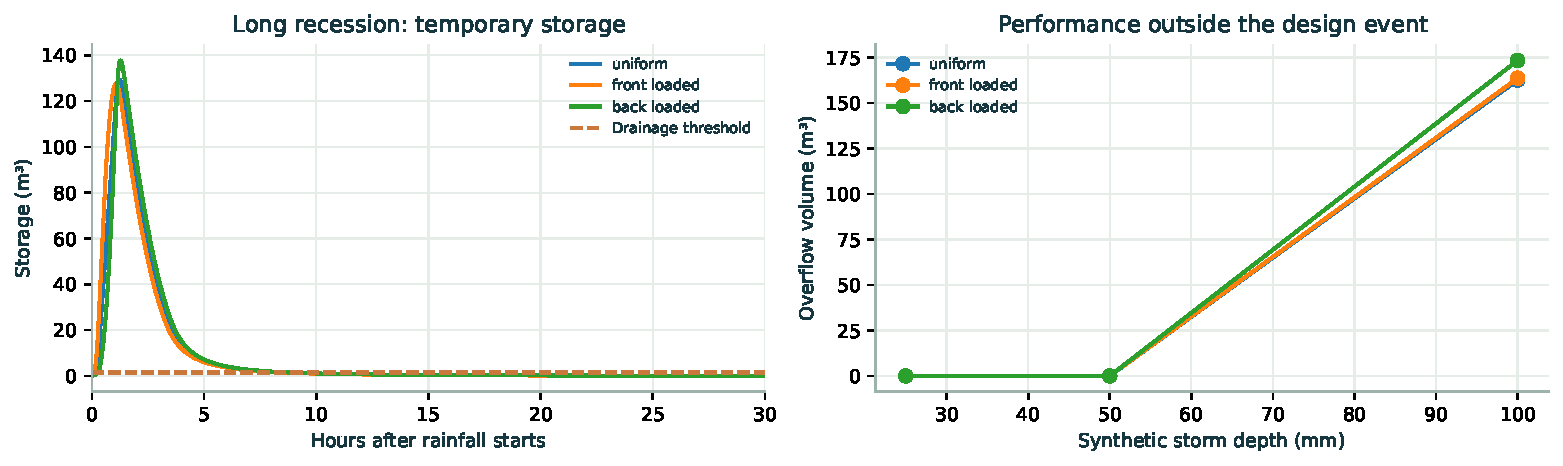
\includegraphics[width=\linewidth,height=2.6in,keepaspectratio]{results/figures/drawdown_and_overflow.pdf}\end{center}
{\footnotesize Figure 4. The drainage threshold corresponds to 7.50 mm of water over the fixed area for the illustrated design. Near the floor the partly wetted outlet produces a long, low-flow tail. The right plot shows excess water once storage is exhausted.}
\newpage
\pagetitle{Verification and sensitivity}
\textbf{Independent calculations.} 16 automated tests cover zero and sub-abstraction rainfall, CN 100, blocked outlets, insufficient storage, full-tail unit-hydrograph timing and volume, and water balance at each step. The outlet integral also matches independent numerical quadrature. For shallow drainage, $Q=kh^{3/2}$ gives the exact no-inflow solution
\[
h(t)=\left[h_0^{-1/2}+kt/(2A_b)\right]^{-2},\qquad k=\tfrac23 C_da\sqrt{2g}.
\]
The numerical solution approaches this limit under step refinement. The workbook separately evaluates CN volume formulas, an exact blocked-storage fixture, and 45 spreadsheet bisection iterations for one controlled-outlet step. Formula caches are re-evaluated from the saved Excel formulas; no manual Excel review is claimed.

\textbf{Water balance.} The largest absolute discrepancy across generation, transformation and routing in the nominal and sensitivity cases is 1e-09 m$^3$. The acceptance tolerance is 0.1\% relative plus $10^{-8}$ m$^3$ absolute. End storage is never silently discarded.

\begin{center}\small\begin{tabular}{rrrrr}\toprule
Steps (s) & Max. peak change (\%) & Max. storage change (\%) & Max. overflow change (m$^3$) & Max. drawdown change (s) \\\midrule
30 $\to$ 15 & 9.0505 & 0.2712 & 0.4377 & 67.25 \\
15 $\to$ 7.5 & 3.5158 & 0.1367 & 0.2180 & 33.57 \\
7.5 $\to$ 3.75 & 3.4323 & 0.0686 & 0.1095 & 16.77 \\
3.75 $\to$ 1.875 & 0.9078 & 0.0342 & 0.0547 & 8.39 \\
\bottomrule\end{tabular}\end{center}
{\footnotesize Changes are maxima across the complete candidate grid, not only the winner. The final two resolutions satisfy the 1\% target for peak and storage; selection and pass/fail decisions are stable. Maximum final overflow-onset movement is 1.875 s. Overflow volume and drawdown differences are reported separately above.}

\textbf{One-at-a-time uncertainty.} The selected geometry is held fixed. Each parameter value is run through all design-event shapes; baseline runoff is recomputed with that parameter. The table reports the worst value for each metric, which may occur in different shapes. The nominal scenario repeats in each parameter group.
\begin{center}\small\begin{tabular}{lrrrrl}\toprule
Varied parameter & Value & Min. reduction (\%) & Max. overflow (m$^3$) & Max. drawdown (h) & All shapes \\\midrule
curve number & 95 & 64.37 & 0.000 & 7.52 & Pass \\
curve number & 98 & 63.09 & 0.000 & 7.81 & Pass \\
curve number & 100 & 47.25 & 2.841 & 7.95 & Fail \\
lag min & 5 & 62.47 & 0.000 & 7.71 & Pass \\
lag min & 10 & 63.09 & 0.000 & 7.81 & Pass \\
lag min & 15 & 63.40 & 0.000 & 7.90 & Pass \\
discharge coefficient & 0.5 & 69.16 & 0.000 & 9.72 & Pass \\
discharge coefficient & 0.62 & 63.09 & 0.000 & 7.81 & Pass \\
discharge coefficient & 0.75 & 57.01 & 0.000 & 6.42 & Pass \\
\bottomrule\end{tabular}\end{center}
These are illustrative parameter bounds, not measured local uncertainty ranges. A sensitivity failure limits the recommendation's robustness; it does not retroactively change the nominal selection rules.
\newpage
\pagetitle{Recommendation, limitations, and review record}
\textbf{Conditional recommendation.} The smallest tested feasible capacity is 150 m$^3$: 0.75 m modeled storage depth over 200 m$^2$, with a 100 by 100 mm floor opening. Across all 50 mm storm shapes, peak reduction is at least 63.09\%, overflow is zero, and the longest drainage time is 7.81 h after rainfall ends. The search establishes the smallest passing \emph{tested} capacity; it is not a continuous optimization or a construction-ready design. A capacity between the tested increments has not been optimized.

\textbf{Limits of the finding.} No site survey, soils investigation, observed rainfall-runoff record or calibration is available. Synthetic depths carry no recurrence interval or location-specific regulatory meaning. CN and lag simplify parking drainage; free discharge excludes tailwater and pipe-network effects. A constant-area basin does not establish safe side slopes or retaining-wall details. There is no freeboard allowance, spillway sizing, water-quality assessment, structural design, infiltration benefit or inundation map. These exclusions constrain how the reported capacity can be interpreted.

\textbf{Reproduction.} Run \texttt{python run\_project.py} in the documented Python environment with pdfLaTeX available. All numerical inputs are local. The command verifies the model, refines the grid, regenerates saved time series, runs sensitivity, and rebuilds the dashboard, workbook, SVG/DXF drawings, figures and this six-page report. Actual runtime, machine architecture, package versions, source hashes and artifact checks are in \texttt{results/run\_manifest.json}. The study-stage runtime in this run was 301.60 s on arm64.

\textbf{Assistance and actual contributions.} Codex implemented, executed, checked and documented the study from the supplied project plan. This report does not attribute model coding, manual Excel verification or CAD editing to Manasi. Her learning guide reserves three review sessions: reproduce a worked check, change an assumption and interpret the result, and inspect/edit the drawing and explain a design choice. Her own written interpretation and sign-off remain pending. Resume wording should reflect her demonstrated contribution after that review.

\textbf{Recorded findings.} The companion \texttt{FINDINGS.md} includes all selected-case metrics, failure mechanisms, sensitivity outcomes, actual execution measurements and outstanding human review. \texttt{CONTRIBUTIONS.md} records assistance explicitly.

{\footnotesize
\begin{thebibliography}{9}
\bibitem{cn}USACE HEC-HMS Technical Reference: SCS Curve Number Loss Model. \href{https://www.hec.usace.army.mil/confluence/hmsdocs/hmstrm/canopy-surface-infiltration-and-runoff-volume/infiltration/scs-curve-number-loss-model}{cn source link}. Accessed 2026-09-08.
\bibitem{uh}USACE HEC-HMS Technical Reference: SCS Unit Hydrograph Model. \href{https://www.hec.usace.army.mil/confluence/hmsdocs/hmstrm/transform/scs-unit-hydrograph-model}{uh source link}. Accessed 2026-09-08.
\bibitem{ordinates}TxDOT Hydraulic Design Manual: NRCS Dimensionless Unit Hydrograph, Table 4-29. \href{https://www.txdot.gov/manuals/des/hyd/chapter-4--hydrology/section-13--hydrograph-method/nrcs-dimensionless-unit-hydrograph.html}{ordinates source link}. Accessed 2026-09-08.
\bibitem{routing}USACE HEC-HMS Technical Reference: Reservoir Modeling Concepts and Equations. \href{https://www.hec.usace.army.mil/confluence/hmsdocs/hmstrm/reservoir-modeling/reservoir-modeling-concepts-and-equations}{routing source link}. Accessed 2026-09-08.
\bibitem{outlet}USACE HEC-HMS User's Manual: Outflow Structures Routing. \href{https://www.hec.usace.army.mil/confluence/hmsdocs/hmsum/latest/reservoir-elements/outflow-structures-routing}{outlet source link}. Accessed 2026-09-08.
\bibitem{selection}TxDOT Hydraulic Design Manual: Selection of the Appropriate Method for Calculating Runoff. \href{https://www.txdot.gov/manuals/des/hyd/chapter-4--hydrology/section-7--selection-of-the-appropriate-method-for.html}{selection source link}. Accessed 2026-09-08.
\end{thebibliography}}
\end{document}
